\documentclass[letterpaper,11pt]{article}


%packages - these add different functionality, and there are many more
\usepackage{amsfonts}
\usepackage{graphicx}
\usepackage[left=2cm,top=2cm,right=2cm,bottom=1.5cm,head=.5cm,foot=.5cm]{geometry}
\usepackage{url}
\usepackage{multirow}
\usepackage{longtable}
\usepackage{subfig}
\usepackage{float}
\usepackage{setspace}
\usepackage{lineno}
\usepackage{natbib}
\usepackage{amsmath}
\usepackage{authblk}
\usepackage{xr}
\usepackage{relsize}
\usepackage{tikz}

%\documentclass[letterpaper,11pt]{article}


%packages - these add different functionality, and there are many more
\usepackage{amsfonts}
\usepackage{graphicx}
\usepackage[left=2cm,top=2cm,right=2cm,bottom=1.5cm,head=.5cm,foot=.5cm]{geometry}
\usepackage{url}
\usepackage{multirow}
\usepackage{longtable}
\usepackage{subfig}
\usepackage{float}
\usepackage{setspace}
\usepackage{lineno}
\usepackage{natbib}
\usepackage{amsmath}
\usepackage{authblk}
\usepackage{xr}
\usepackage{relsize}
\usepackage{tikz}
\usepackage{hyperref}

%\documentclass[letterpaper,11pt]{article}


%packages - these add different functionality, and there are many more
\usepackage{amsfonts}
\usepackage{graphicx}
\usepackage[left=2cm,top=2cm,right=2cm,bottom=1.5cm,head=.5cm,foot=.5cm]{geometry}
\usepackage{url}
\usepackage{multirow}
\usepackage{longtable}
\usepackage{subfig}
\usepackage{float}
\usepackage{setspace}
\usepackage{lineno}
\usepackage{natbib}
\usepackage{amsmath}
\usepackage{authblk}
\usepackage{xr}
\usepackage{relsize}
\usepackage{tikz}
\usepackage{hyperref}

%\documentclass[letterpaper,11pt]{article}


%packages - these add different functionality, and there are many more
\usepackage{amsfonts}
\usepackage{graphicx}
\usepackage[left=2cm,top=2cm,right=2cm,bottom=1.5cm,head=.5cm,foot=.5cm]{geometry}
\usepackage{url}
\usepackage{multirow}
\usepackage{longtable}
\usepackage{subfig}
\usepackage{float}
\usepackage{setspace}
\usepackage{lineno}
\usepackage{natbib}
\usepackage{amsmath}
\usepackage{authblk}
\usepackage{xr}
\usepackage{relsize}
\usepackage{tikz}
\usepackage{hyperref}

%\input{../paper/writeup.tex}
\externaldocument[SI-]{SI}
\input{../results/NumericResults.tex}

%header material for paper delineated below but not actually run until \maketitle in the main document body
\title{Genome size as a prediction of plant adaptation across environments}
\date{}

\author[a,*]{Linh Nguyen}
\author[a]{Daniel C. Reuman}

\affil[a]{Department of Ecology and Evolutionary Biology and Center for Ecological Research, University of Kansas}
\affil[*]{Corresponding author, l233n428@ku.edu}

%This starts the actual body of the paper
\begin{document}

%adds linenumbers, good for submitting papers
\linenumbers

%actually creates the title, affiliations, etc in pdf
\maketitle

% get abstract
\begin{abstract}
\noindent Genome size is an important factor of evolutionary since it relies on how chromosomes
will eventually fold and express, and then to its genotypes and phenotypes. 
It has been debated with multiple hypotheses to explain genome size variation,
from the influence from evolutionary history to environments and adaptation. 

\noindent In this assignment, I examined genome size using lars2 to investigate factors 
that contribute to its variation and if they harbor linear relationship
to genome size or not.
\end{abstract}

\section{Introduction}\label{section:introduction}
Genome size has been an important factor of genome. Angiosperm species exhibit a wide range of variation in genome size
that many hypotheses have been proposed to explain the variation. 

\section{Methods}\label{section:methods}
We use lars2 package from caret to examine relationship between genome size and other factors.

We proposed a model of genome size, that genome size is explainable through range size and bioclimatic variables
\[ \log_{10}(\text{Genome size}) \sim \log_{10}(\text{Range size}) + \text{number of chromosome} + \text{Bioclimatic variables} \]

Here, Genome size is the genome size of species recorded in this dataset and the response variable that we are interested in.
Range size is the range size of species recorded, number of chromosome is the number of chromosome of that speices, 
and Bioclimatic variables are reported in SI. 

See SI section \ref{SI-SIsect:reiter} for more details on bioclimatic variables.



\section{Results}\label{section:results}

On the training set, lars2 had an RMSE of $\rmsetrain$ and an $R^2$ of \rsquaretrain.
Then, we tunned the trained model with more steps at it did not improve the performance with 
RMSE of $\rmsetune$ and an $R^2$ of \rsquaretune. 
Hence, we used intial model to test on test set.
On the test set, it had an RMSE of $\rmsetest$ and an $R^2$ of \rsquaretest.

The tuning graph of tuning process is reported here:
\begin{figure}
%This part brings the pdf figure in
\centering
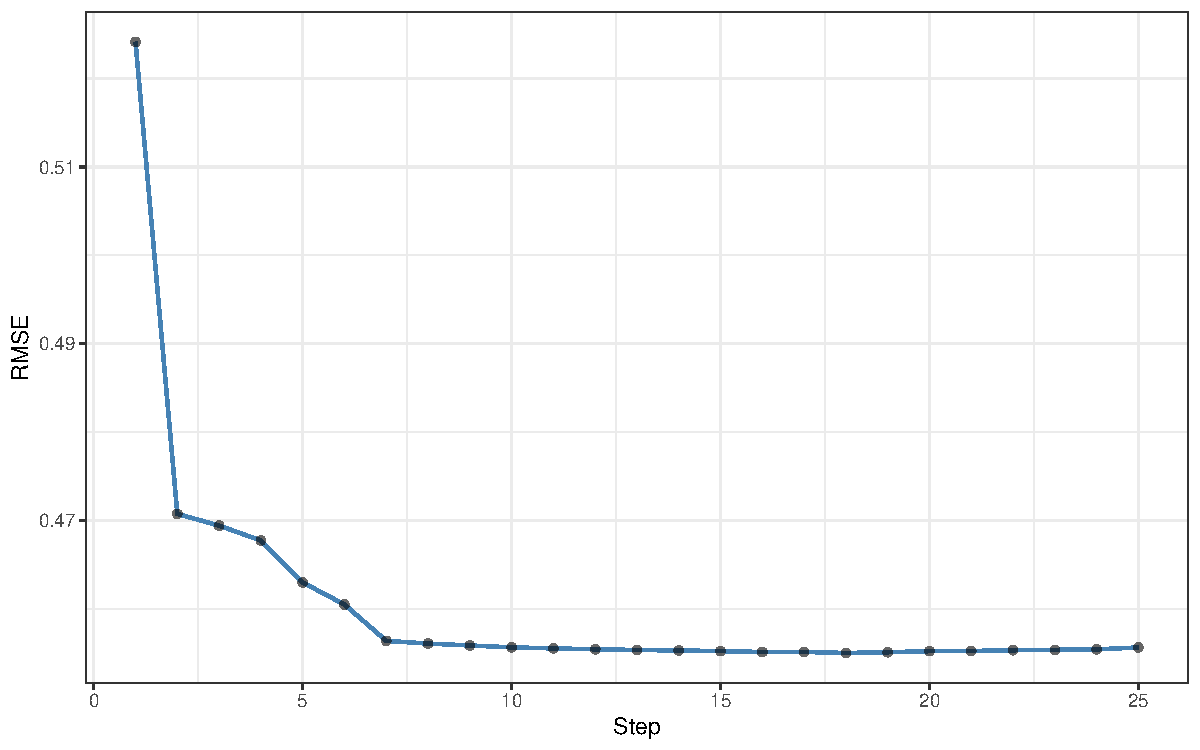
\includegraphics[width=0.6\textwidth]{../results/RMSE_dist_lars2.pdf}
%The caption. Note the numeric result can be used here too.
\caption{Tuning steps of lars2 and corresponding RMSE of each step}
\end{figure}



\end{document}
\externaldocument[SI-]{SI}
\newcommand{\rmsetrain}{0.453}
\newcommand{\rsquaretrain}{0.247}
\newcommand{\rmsetest}{0.462}
\newcommand{\rsquaretest}{0.233}
\newcommand{\rmsetune}{0.455}
\newcommand{\rsquaretune}{0.019}

%header material for paper delineated below but not actually run until \maketitle in the main document body
\title{Genome size as a prediction of plant adaptation across environments}
\date{}

\author[a,*]{Linh Nguyen}
\author[a]{Daniel C. Reuman}

\affil[a]{Department of Ecology and Evolutionary Biology and Center for Ecological Research, University of Kansas}
\affil[*]{Corresponding author, l233n428@ku.edu}

%This starts the actual body of the paper
\begin{document}

%adds linenumbers, good for submitting papers
\linenumbers

%actually creates the title, affiliations, etc in pdf
\maketitle

% get abstract
\begin{abstract}
\noindent Genome size is an important factor of evolutionary since it relies on how chromosomes
will eventually fold and express, and then to its genotypes and phenotypes. 
It has been debated with multiple hypotheses to explain genome size variation,
from the influence from evolutionary history to environments and adaptation. 

\noindent In this assignment, I examined genome size using lars2 to investigate factors 
that contribute to its variation and if they harbor linear relationship
to genome size or not.
\end{abstract}

\section{Introduction}\label{section:introduction}
Genome size has been an important factor of genome. Angiosperm species exhibit a wide range of variation in genome size
that many hypotheses have been proposed to explain the variation. 

\section{Methods}\label{section:methods}
We use lars2 package from caret to examine relationship between genome size and other factors.

We proposed a model of genome size, that genome size is explainable through range size and bioclimatic variables
\[ \log_{10}(\text{Genome size}) \sim \log_{10}(\text{Range size}) + \text{number of chromosome} + \text{Bioclimatic variables} \]

Here, Genome size is the genome size of species recorded in this dataset and the response variable that we are interested in.
Range size is the range size of species recorded, number of chromosome is the number of chromosome of that speices, 
and Bioclimatic variables are reported in SI. 

See SI section \ref{SI-SIsect:reiter} for more details on bioclimatic variables.



\section{Results}\label{section:results}

On the training set, lars2 had an RMSE of $\rmsetrain$ and an $R^2$ of \rsquaretrain.
Then, we tunned the trained model with more steps at it did not improve the performance with 
RMSE of $\rmsetune$ and an $R^2$ of \rsquaretune. 
Hence, we used intial model to test on test set.
On the test set, it had an RMSE of $\rmsetest$ and an $R^2$ of \rsquaretest.

The tuning graph of tuning process is reported here:
\begin{figure}
%This part brings the pdf figure in
\centering
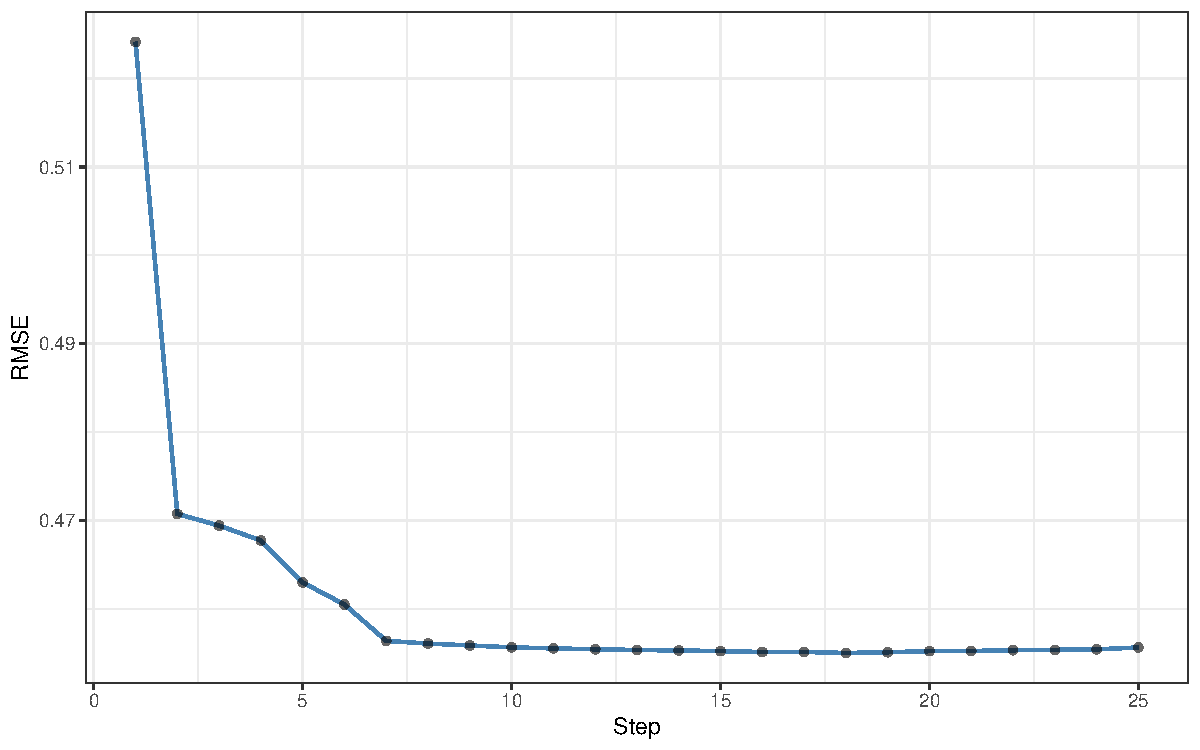
\includegraphics[width=0.6\textwidth]{../results/RMSE_dist_lars2.pdf}
%The caption. Note the numeric result can be used here too.
\caption{Tuning steps of lars2 and corresponding RMSE of each step}
\end{figure}



\end{document}
\externaldocument[SI-]{SI}
\newcommand{\rmsetrain}{0.453}
\newcommand{\rsquaretrain}{0.247}
\newcommand{\rmsetest}{0.462}
\newcommand{\rsquaretest}{0.233}
\newcommand{\rmsetune}{0.455}
\newcommand{\rsquaretune}{0.019}

%header material for paper delineated below but not actually run until \maketitle in the main document body
\title{Genome size as a prediction of plant adaptation across environments}
\date{}

\author[a,*]{Linh Nguyen}
\author[a]{Daniel C. Reuman}

\affil[a]{Department of Ecology and Evolutionary Biology and Center for Ecological Research, University of Kansas}
\affil[*]{Corresponding author, l233n428@ku.edu}

%This starts the actual body of the paper
\begin{document}

%adds linenumbers, good for submitting papers
\linenumbers

%actually creates the title, affiliations, etc in pdf
\maketitle

% get abstract
\begin{abstract}
\noindent Genome size is an important factor of evolutionary since it relies on how chromosomes
will eventually fold and express, and then to its genotypes and phenotypes. 
It has been debated with multiple hypotheses to explain genome size variation,
from the influence from evolutionary history to environments and adaptation. 

\noindent In this assignment, I examined genome size using lars2 to investigate factors 
that contribute to its variation and if they harbor linear relationship
to genome size or not.
\end{abstract}

\section{Introduction}\label{section:introduction}
Genome size has been an important factor of genome. Angiosperm species exhibit a wide range of variation in genome size
that many hypotheses have been proposed to explain the variation. 

\section{Methods}\label{section:methods}
We use lars2 package from caret to examine relationship between genome size and other factors.

We proposed a model of genome size, that genome size is explainable through range size and bioclimatic variables
\[ \log_{10}(\text{Genome size}) \sim \log_{10}(\text{Range size}) + \text{number of chromosome} + \text{Bioclimatic variables} \]

Here, Genome size is the genome size of species recorded in this dataset and the response variable that we are interested in.
Range size is the range size of species recorded, number of chromosome is the number of chromosome of that speices, 
and Bioclimatic variables are reported in SI. 

See SI section \ref{SI-SIsect:reiter} for more details on bioclimatic variables.



\section{Results}\label{section:results}

On the training set, lars2 had an RMSE of $\rmsetrain$ and an $R^2$ of \rsquaretrain.
Then, we tunned the trained model with more steps at it did not improve the performance with 
RMSE of $\rmsetune$ and an $R^2$ of \rsquaretune. 
Hence, we used intial model to test on test set.
On the test set, it had an RMSE of $\rmsetest$ and an $R^2$ of \rsquaretest.

The tuning graph of tuning process is reported here:
\begin{figure}
%This part brings the pdf figure in
\centering
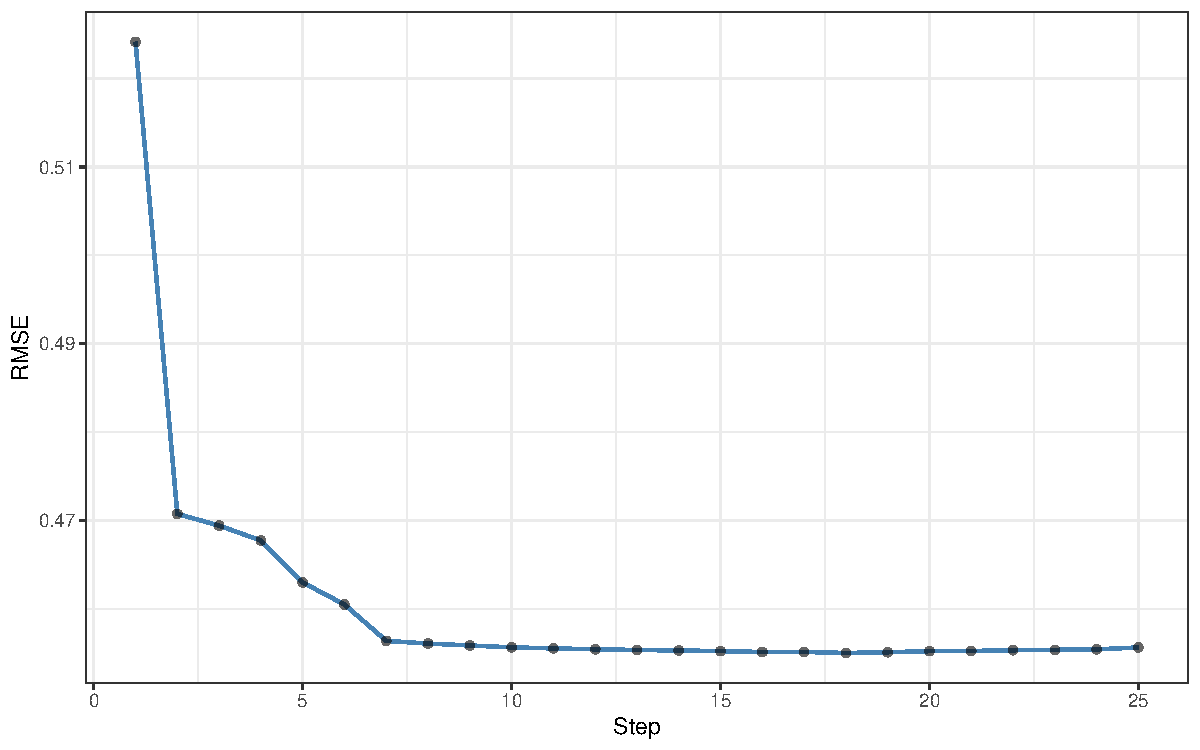
\includegraphics[width=0.6\textwidth]{../results/RMSE_dist_lars2.pdf}
%The caption. Note the numeric result can be used here too.
\caption{Tuning steps of lars2 and corresponding RMSE of each step}
\end{figure}



\end{document}


%header material for paper delineated below but not actually run until \maketitle in the main document body
\title{Supplemental material for "Genome size as a prediction of plant adaptation across environments" paper}
\date{}

\author[a,*]{Linh Nguyen}
\author[a]{Daniel C. Reuman}

\affil[a]{Department of Ecology and Evolutionary Biology and Center for Ecological Research, University of Kansas}
\affil[*]{Corresponding author, l233n428@ku.edu}

%This starts the actual body of the paper
\begin{document}

%adds linenumbers, good for submitting papers
\linenumbers

%actually creates the title, affiliations, etc in pdf
\maketitle

\tableofcontents

\section{Main result reiterated}\label{SIsect:reiter}
Bioclimatic variables were recorded using GBIF dataset, based on location of collected species. 

\begin{table}[ht] 
    \centering 
    \caption{Description of bioclimatic variables} 
    \label{tab:variables} 
    \begin{tabular}{p{4.5cm} p{9cm}} 
        \textbf{Variable} & \textbf{Description} \\ 
        \texttt{log10\_range\_size} & Log$_{10}$-transformed geographic range size (response variable) \\ 
        \texttt{log10\_2C\_genome.size} & Log$_{10}$-transformed 2C genome size \\ 
        \texttt{num\_chr2n} & Diploid chromosome number \\ 
        \texttt{Latitude} & Latitude \\ 
        \texttt{Growth\_form} & Plant growth form \\ 
        \texttt{log10\_occurence} & Log$_{10}$-transformed occurrence \\ 
        \texttt{Longitude} & Longitude \\ 
        \texttt{Mean.aridity.index} & Mean aridity index \\ 
        \texttt{Mean.BIO1} & Mean annual temperature \\ 
        \texttt{Mean.BIO3} & Isothermality \\ 
        \texttt{Mean.BIO7} & Annual temperature range \\ 
        \texttt{Mean.BIO12} & Annual precipitation \\ 
        \texttt{Mean.BIO15} & Precipitation seasonality \\ 
        \texttt{Mean.BIO19} & Precipitation of the coldest quarter \\ 
        \texttt{Mean.GSL} & Growing season length \\ 
        \texttt{Mean.GST} & Temperature during the growing season \\ 
        \texttt{Mean.NGD5} & Number of days with temperature $> 5^\circ$C \\ 
        \texttt{Mean.UVB1} & Annual ultraviolet-B radiation \\ 
        \texttt{Mean.UVB3} & Mean UV-B radiation of the highest month \\ 
        \texttt{Mean.UVB5} & Sum of monthly mean UV-B radiation \\ 
    \end{tabular} 
\end{table}

\end{document}